\section{Abbildungen}

\subsection{Idee:}
Es seien $A$ und $B$ Mengen. Unter einer Abbildung $f$ stellen wir uns einen Algorithmus vor, der aus jeder eingabe $a \in A$ ein eindeutig bestimmte Ausgabe $b \in B$ errechnet, $b$ ist nur durch $a$ (und $f$) festgelegt.

\begin{figure} [H]
\centering 
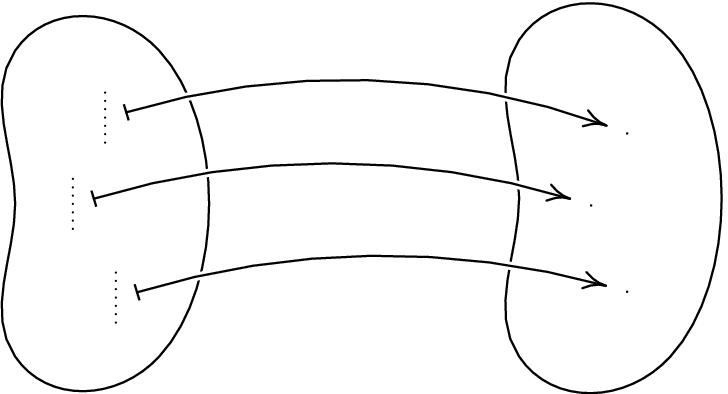
\includegraphics[width=10cm, height=6cm]{mainmatter/chapter1/pics/abbildunggenerell.png}
\caption{Eine einfache Abbildung} 
\end{figure}
%
%
%
\subsection{Definition:}

Es seien $A$ und $B$ Mengen. Eine Abbildung $f$ mit $ f:A \rightarrow B $ sei eine Teilmenge $f$ von $AxB = \{ (a,b) | a \in A, b \in B \}$ so, dass gilt:

\begin{description} 
\item[-] zu jedem $a \in A$ existiert ein $b \in B$ mit $(a,b) \ in f$ 
\item[-] sind $(a,b_{1}), (a,b_{2}) \in f$, so gilt $b_{1} = b_{2}$
\end{description}

$f$ ist also das, was in der Schule im Fall reller Funktionen als Graph der Funktion bezeichnet wurde. Anstatt $(a,b) \in f$ schreiben wir $b = f(a)$. Die Menge $A$ heißt Definitionsbereich von $f$, die Menge $B$ heißt Zielbereich von $f$. Ferner sei Bild $f = \{b \in B | \exists a \in A$ mit $f(a) = b\} = \{f(a) |  a \in A\} = f(A))$ (Wertebereich)
%
%
%
\subsection{Beispiel:}
	\begin{enumerate} 

		\item Vorzeichenfunktion $sign.$ $\mathbb{Z} \rightarrow\{-1,0,1\}$ $sign= \{(z,1)|z < 0\} \cup \{(0,0)\} \cup \{(z,1)|z > 0\}$

		\item  Identität: Für jede Menge $A$ sei $id_{A}: A \rightarrow A$ gegeben durch $id_{A} (b)=a$ $ \forall a \in A$

		\begin{description}
			\item[ ]{\pgreen $f:\mathbb{R}\rightarrow \mathbb{R}$, $f(a) = a^{2}$ $\forall a \in \mathbb{R}$}
			\item[ ]{\pblue $g:\mathbb{R}\rightarrow \mathbb{R}$, $g(a)=2a$ $\forall a\in \mathbb{R}$}
				\begin{figure} [H]
				\centering 
				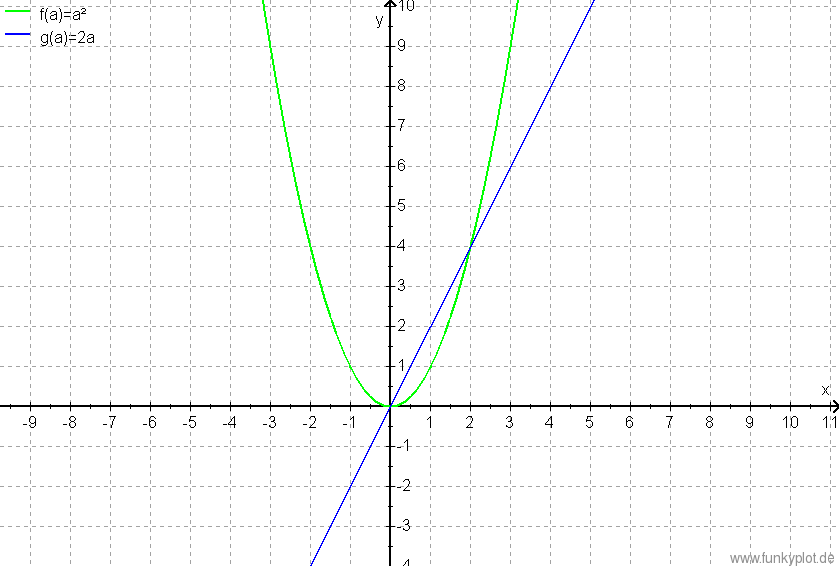
\includegraphics[width=14cm, height=8cm]{mainmatter/chapter1/pics/graph.png}
				\caption{Ein Beispiel Graph} 
				\end{figure}
			\item[ ] Bild $f=\{b \in \mathbb{R} | b \geq 0\} \subsetneqq \mathbb{R}$
			\item[ ] Bild $g = \mathbb{R}$
		\end{description}
		
		\item $g:\mathbb{Z}\rightarrow\mathbb{Z}$, $g(a)=\{2a|a\in\mathbb{Z}\} \subsetneqq \mathbb{Z}$ (Kurzschreibweise: $(=2\mathbb{Z})$)

	\end{enumerate} 
%
%
%
\subsection{Definition:}
Eine Abbildung $f: A \rightarrow B$ heiße:

	\begin{description}
		\item[-] surjektiv, falls Bild $f = B$ ist d.h., falls $\forall b \in B$ ein $a \in A$ existiert mit $f(a)=b$


		\item[-] injektiv, falls es zu jedem $b \in B$ höchstens ein $a \in A$ gibt mit $f(a)=b$.
		\begin{description}
			\item[] d.h.
			\item[-]  aus $f(a_{1}) = f(a_{2})$ folgt $a_{1}=a_{2}$
			\item[-] aus $a_{1} \neq a_{2}$ folgt $f(a_{1}) \neq f(a_{2})$
		\end{description}
		
		\item[-] bijektiv, falls $f$ injektiv und surjektiv ist 
				\begin{figure} [H]
				\centering 
				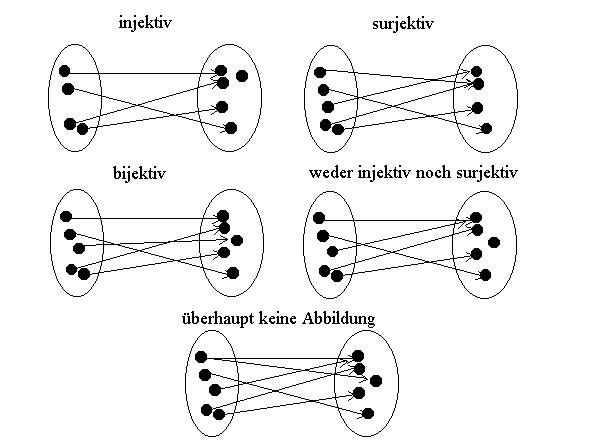
\includegraphics[width=17cm, height=10cm]{mainmatter/chapter1/pics/abbildungen.jpg}
				\caption{Mögliche Abbildungen auf einen Blick} 
				\end{figure}
	\end{description}


%
%
%
\subsection{Beispiel:}
	Sei $\mathbb{R}_{\geq0}=\{a \in \mathbb{R}|a \geq 0\}$
	\begin{enumerate}
		\item $f: \mathbb{R} \rightarrow \mathbb{R}$, $f(a)=a^{2}$ nicht surjektiv, nicht injektiv $(-1 \notin$ Bild $f)$ $((-1)^{2} = 1^{2})$
		\item $f: \mathbb{R} \rightarrow \mathbb{R}_{\geq0}$, $f(a) = a^{2}$ surjektiv, nicht injektiv
		\item $f: \mathbb{R}_{\geq0} \rightarrow \mathbb{R}$, $f(a) = a^{2}$ nicht surjektiv, injektiv
		\item $f: \mathbb{R}_{\geq0} \rightarrow \mathbb{R}_{\geq0}$, $f(a) = a^{2}$ bijektiv
	\end{enumerate}
%
%
%
\subsection{Definition}
\subsubsection{Komposition von Abbildungen }

Es seien $f: A \rightarrow B$ und $g: B\rightarrow C$ Abbildungen. 
Wir definieren $g \circ f: A\rightarrow C$ vermöge $(g \circ f) (a) = g(f(a))$ $\forall a\in A$
				\begin{figure} [H]
				\centering
				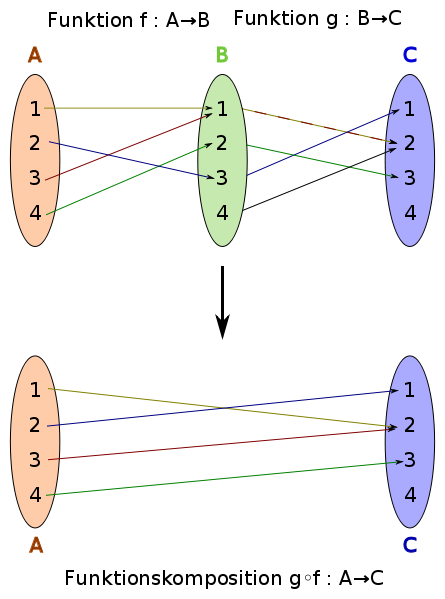
\includegraphics[width=6cm, height=8cm]{mainmatter/chapter1/pics/komposition.png}
				\caption{Eine mögliche Komposition} 
				\end{figure}
%
%
%
\subsection{Beispiel}
$f,g: \mathbb{R} \rightarrow \mathbb{R}$, $f(x)=x^{2}$, $g(x)=2x$ $\forall x \in \mathbb{R}$ 
	\begin{description}
		\item[] Dann:
		\begin{description}
			\item[] $(g \circ f)(x) = g(f(x)) = g(x^{2}) = 2x^{2}$
			\item[] $(f \circ g)(x) = f(g(x)) = f(2x) = (2x)^{2} = 4x^{2}$
		\end{description}
	\end{description}
Es kommt auf die Reihenfolge von f und g an!
%
%
%
\subsection{Satz}

Seien $f: A \rightarrow B$ und $g:B \rightarrow A$ Abbildungen mit $g \circ f = id_{A}$ Dann ist $f$ injektiv und $g$ surjektiv.

	\subsubsection{Beweis:}
		$f$ injektiv: Seien $a_{1},a_{2} \in A$ mit $ f(a_{1}) = f(a_{2}) $ z.z. $a_{1} = a_{2}$
		\begin{description}
			\item[]  Dazu: $a_{1} = id_{A}(a_{1}) = (g \circ f) (a_{1}) = g(f(1_{1})) = g(f(a_{2})) = (g \circ f)(a_{2}) = id_{A} (a_{2}) = a_{2}$
			\item[] g surjektiv: Sei $a \in A$ (=Zielbereich von g)
			\item[] z.z. Es gibt ein $b \in B$ (=Definitionsbereich von g) mit $g(f(a)) = (g \circ f)(a) = id_{A}(a) = a$ wähle daher $b=f(a)$
		\end{description}
	/* $f: A \rightarrow B$\qquad $ f\circ id_{A}:A\rightarrow B$\qquad $f\circ id_{A}=f$ */

\subsection{Definition:}
	In der Situation I.1.8 nennen wir $g$ eine linksinverse von $f$ und $f$ eine rechtsinverse von $g$.

\subsection{Definition:}
	Ist $f: A \rightarrow B$ bijektiv, so sei die zu $f$ inverse Abbildung $f^{-1}: B \rightarrow A$ gegeben durch $f^{-1} = \{ (b,a) \in B$x$A| a,b \in f\}$

		\begin{description}
			\item[Warnung:] Das klappt nur bei bijektiven Abbildungen $f$, da $f_{-1}$ beidseitig invers zu $f$ ist. 
			\item[Hinweis:] $f^{-1}$ inverse der Abbildung \qquad $f1^{-}$ volles Urbild jedoch ist dies nicht zwangsläufig bijektiv
		\end{description}

\subsection{Definition:}
	Sei $f:A \rightarrow B$ und $Y \leq B$. Dann nennen wir $j(Y) = \{ a \in A | f(a) \in Y\}$ das volle Urbild zu $Y$ unter $f$. 

		\begin{figure} [H]
		\centering 
		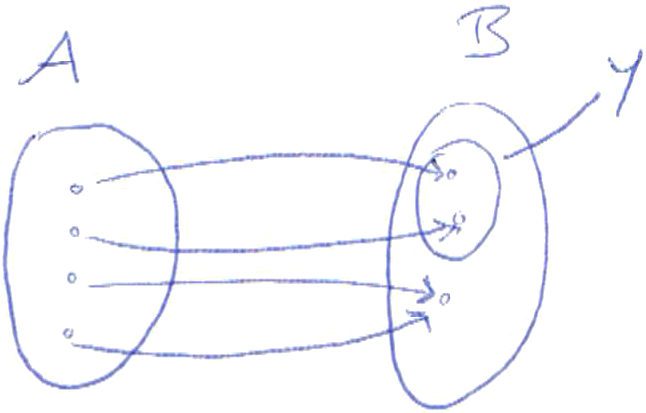
\includegraphics[width=5cm, height=3cm]{mainmatter/chapter1/pics/untermengen1.png}
		\caption{Eine Abbildung auf Untermengen} 
		\end{figure}
\subsection{Beispiel:}
In 1.5(1) war $f: \mathbb{R} \rightarrow \mathbb{R}$, $f(a)=a^{2}$.
$f(\{0,1,4\}) = \{-2,-1,0,1,2\}$

\begin{description}

	\item[Beispiel:] $g:\mathbb{Z} \rightarrow \mathbb{Z}$, $g(a)=a^{2}$ \\
	$f^{-}(\{0,1,2,3,4\}) = \{-2,-1,0,1,2\}$

\end{description}
